\begin{figure}
\caption{An example configuration of the scene}
\centering
\label{fig:scene}
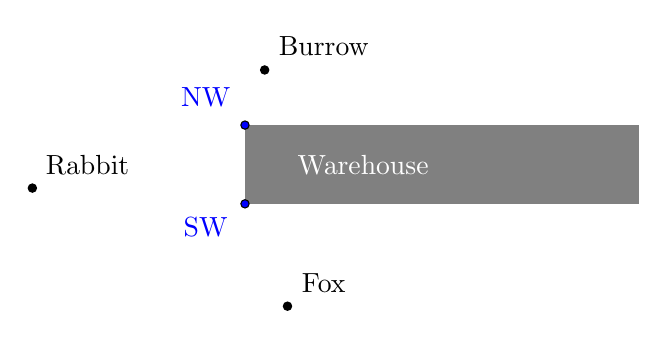
\begin{tikzpicture}  

\fill (3,3) [gray] rectangle (8,4);

\filldraw (3.25,4.7) circle[radius=1.5pt];
\filldraw (0.3,3.2) circle[radius=1.5pt];
\filldraw (3.54,1.7) circle[radius=1.5pt];

\filldraw[fill=blue] (3,3) circle[radius=1.5pt];
\filldraw[ fill=blue] (3, 4) circle[radius=1.5pt];

\node[] at (4,5) {Burrow};
\node[] at (1,3.5) {Rabbit};
\node[] at (4,2) {Fox};

\node[ text=blue] at (2.5,4.35) {NW};
\node[ text=blue] at (2.5,2.7) {SW};

\node[text=white, draw=gray] at (4.5,3.5) {Warehouse};

\end{tikzpicture}
\end{figure}